\documentclass[10pt,a4paper]{article}
\usepackage{amsmath}
\usepackage{amsfonts}
\usepackage{amssymb}
\usepackage{CJK}													% 支持中文
\usepackage{indentfirst}                 						% 首行缩进宏包
\usepackage{graphicx}											% 支持图片的插入
\usepackage{subfigure}											% 支持插入子图
\usepackage[colorlinks,citecolor = blue, linkcolor=blue,hyperindex,CJKbookmarks]{hyperref}	% 链接功能
\usepackage{CJKfntef}

\graphicspath{{figs/}}                              				% 图片文件夹路径
\setlength{\parindent}{2em}										% 缩进距离为2个字符位置
\newcommand{\song}{\CJKfamily{song}}     						% 宋体
\newcommand{\hei}{\CJKfamily{hei}}       						% 黑体
\newcommand{\fs}{\CJKfamily{fang}}         						% 仿宋
\newcommand{\kai}{\CJKfamily{kai}}       						% 楷体
\newcommand{\li}{\CJKfamily{li}}         						% 隶书
\newcommand{\you}{\CJKfamily{you}}       						% 幼圆

\begin{document}

\begin{CJK*}{UTF8}{gkai}
%============================++题目和作者++================================
\title{贝叶斯网络学习指南}					   					% 题目
\author{David Heckerman		\\  
        heckerma@microsoft.com \\
        \\
        March 1995(Revised November 1996)\\
        \\
        Technical Report\\
		}
%============================++++++++++++=================================
\date{}                                             				% 显示作者,不显示日期
\maketitle                                          				% 生成标题
\clearpage
\tableofcontents 												% 生成目录
\clearpage


%============================++摘要和关键字++===============================
\newcommand{\cnabstract}
{
贝叶斯网络是一个图模型,能够将一系列变量之间的关系以图的形式表现出来。当它结合统计技术进行数据分析时有下列优点。第一,因为模型能体现各个变量的依赖关系,所以它能够处理部分数据缺失的情况。第二,贝叶斯网络可以用来学因果关系,因此能够加深对问题的理解并预测结果。第三,因为该模型既包含因果也包含概率语义,所以它是先验知识和数据的理想表示。第四,贝叶斯统计方法结合贝叶斯网络能有效的避免数据的过拟合。在这篇论文中, 我们将讨论由先验知识构建贝叶斯网络的方法并且将数据通过贝叶斯统计学方法来优化该模型。至于后面的任务,我们介绍了贝叶斯网络的参数学习和结构学习,其中包含了从不完全的数据中去学习。此外,我们将贝叶斯网络的学习和监督和非监督学习联系起来。最后我们介绍了图模型在真实世界的案例分析。
}
\newcommand{\cnkeywords}{贝叶斯网络,贝叶斯统计方法,参数学习,结构学习}
%============================++++++++++++=================================
\begin{center}
\begin{minipage}[c]{12cm}										% 小页环境-摘要
\hei 摘要:\kai \cnabstract\\
\hei 关键字:\kai \cnkeywords\\
\end{minipage}
\end{center}
\newpage



%================================主体====================================
\section{引言}
贝叶斯网络是一个表示一系列变量之间的概率关系的图模型。在过去的十年,贝叶斯网络成为了对专家系统中不确定的专家知识描述的最流行的代表。最近研究人员研发出很多从数据中学习贝叶斯网络的方法。这些技术是崭新的并且仍然在发展,但是对一些数据分析问题,他们已经表现出优异的性能。


在这篇文章中,我们介绍了贝叶斯网络和从数据中提取和描述知识的相关贝叶斯方法的学习指南。\marginpar{\small 这里代表和方法怎么区分,分类对不?}\CJKunderwave*{数据分析的代表(representations)有很多,包括规则库、决策树和神经网络。也有很多数据分析的方法,像密度估计、分类、回归和聚类}。所以贝叶斯网络和贝叶斯方法能够干什么?这里至少有四个答案。


\marginpar{\small 样例需要进一步丰满}第一,贝叶斯网络可以有效的处理不完全数据集。举个例子,一个分类或回归问题:有两个变量是完全反相关。当每个样例中所有变量都是可测量的,对于标准的监督学习技术,这种相关关系很容易判别出来。然而,当其中一个变量是不可观察的,大部分模型将会得出一个不准确的预测,因为它们无法计算两个输入变量之间的关系。而贝叶斯网络能够提供一个自然的方法来表示这种依赖关系。


第二,贝叶斯网络可以学习因果关系。这里有两个原因来说明学习因果关系的重要性。首先,学习的过程很有用,特别是我们在数据分析中尝试弄明白问题时。此外,因果关系的知识可以让我作预测,无论由因推果还是由果推因。举个例子,市场分析师可能想要知道为了提高销量,通过特别的广告来提高产品曝光率行不行。为了解决这个问题,分析师可以通过贝叶斯网络来确定产品销量提高的原因有没有广告因素,如果有,这个因素对销量的影响到了什么程度。甚至没有提高曝光度的影响的试验也是可行的(第一个优点--处理不完全数据集)。


第三,结合了贝叶斯统计方法的贝叶斯网络促进了先验知识和数据的结合。在现实世界里做分析的人知道先验知识或领域知识的重要性,特别是当数据要么稀少要么昂贵的时候。一些商业系统,像专家系统可以单独由先验知识构建。这个事实是对先验知识重要性的验证。贝叶斯网络有因果的语义,能够直接由先验知识直接构建。此外,贝叶斯网络能够用概率来描述因果关系。最终,先验知识和数据可以和贝叶斯统计方法很好的结合起来。


第四,\marginpar{\small 怎么就避免过拟合了?}\CJKunderwave*{结合了贝叶斯方法的贝叶斯网络和其他模型能有效的避免数据的过拟合}。由此,\marginpar{\small 测试的目的是为了对模型的一种检验和衡量,个人认为不可缺少。}\CJKunderwave*{没有必要拿出一些数据来测试。用贝叶斯方法,模型将会很平滑以至于所有数据都可以用来训练}。


下面介绍一下这篇文章的结构组织。第二部分,我们讨论一下概率的贝叶斯解释并且复习一下结合先验知识和数据的贝叶斯统计方法。第三部分,我们描述了贝叶斯网络并且讨论它如何只通过先验知识来构建。第四部分,我们讨论一下在贝叶斯网络里面的概率推理算法。第五和第六部分,我们学习如何在固定的贝叶斯网络结构中学习概率并且描述了包括Monte-Carlo
方法和Gaussian方法来处理不完全数据的技术。第七到十二部分,我们介绍贝叶斯网络的参数学习和结构学习。其中对于贝叶斯网络参数学习和结构学习的评估方法还有对Monte-Carlo、Laplace、BIC和MDL这些算法如何避免数据的过拟合进行了讨论。第十三和十四部分,我们描述了贝叶斯网络和监督及非监督学习的关系。第十五部分,我们介绍贝叶斯网络促进了因果关系的学习。第十六部分,我们结合真实世界的案例用指南中的方法进行了分析解决。第十七部分,我们给出了软件和其他论文的链接。



\section{概率和统计的贝叶斯方法}
为了学习贝叶斯网络和相关的学习方法,理解概率和统计的贝叶斯方法。在这部分,我们为只熟悉古典概率的人介绍一下贝叶斯方法。

简而言之,\textbf{一个事件$x$的贝叶斯概率}是指\textcolor{blue}{一个人对事件$x$的信任程度},它是分配概率那个人的属性(比如你对抛置一枚硬币正面朝上事件的信任程度)。而\textbf{古典概率}是\textcolor{blue}{世界的物理属性}(比如抛置一枚硬币正面朝上的概率)。为了保证这两个概念可分,我们称一个事件的古典概率为事件的真实概率或物理概率,而称一个事件的信任程度为贝叶斯概率或个人概率。在本文里,我们常将贝叶斯概率简称为概率。




物理概率和个人概率最大的区别是测量个人概率我们不需要重复的试验。比如,想象重复的将糖块投掷在湿地上。每次糖块被投掷后,它将会轻微形变。因此,古典概率测量糖块某个面朝上的概率是很困难的,但是贝叶斯只关注下一次投掷,并且给出概率。这里有另一个样例,考虑一个问题:在2001年芝加哥公牛队夺得下一次冠军的概率是多少。这里,古典统计学者肯定会保持沉默,然后贝叶斯可以给出一个概率(可能还可以从中小赚一小笔)。


贝叶斯概率的定义常受到质疑,其中一个就是概率变得模棱两可。信任程度如何满足概率的定义(rules of propability
\footnote{概率定义:设随机事件的样本空间为$\Omega$,对于$\Omega$中的每一个事件$A$,都有实函数$P(A)$满足1)非负性:$P(A)\geq0$; 2)规范性:$P(\Omega)=1$; 3)可加性:对n个两两互斥事件$A_1,\cdots,A_n$有:$\sum_{i=1}^n P(A_i)=P(\bigcup_{i=1}^n A_i)$,任意一个满足上述条件的函数P都可以作为样本空间$\Omega$的概率函数,称函数值$P(A)$为$\Omega$中事件$A$的概率。})?
而概率应该在哪种标准下衡量?特别的,我们知道必然(不)发生的事件的贝叶斯概率是1(0),但是对于不是这两种特例情况的事件又如何衡量事件发生的概率呢?不用惊讶,这些问题已经被深刻的研究了。


至于第一个问题,\marginpar{\small many researchers have suggested different sets of properties that should be satisfied by degrees of belief}\CJKunderwave*{许多研究者建议不同属性集应该满足信任程度}(Ramsey 1931, Cox 1946, Good 1950, Savage 1954, DeFinetti 1970)。结果是每个属性集产生相同的规则:概率规则。虽然每个属性集是强制的,但是不同的属性集将产生概率规则的事实是使用概率来衡量信任程度的强有力证据。


程度问题的答案来自一个简单的观察:人们很容易发现两个事件的概率差不多。比如,想象一个简化的只有两个区域(阴影和非阴影)的幸运转盘,就像在图\ref{fig:wheel}所示。
\begin{figure}[!htbp]
	\centering
    	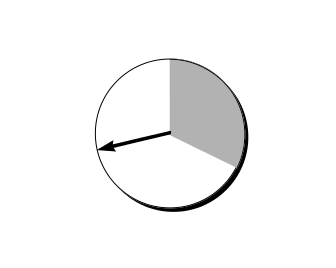
\includegraphics[scale=0.4]{figs/wheel.png}
	\caption{概率转盘:用来衡量概率的工具}    
	\label{fig:wheel}
\end{figure}
假定转盘是完全对称的(除了底纹),可以看出转盘停在任何位置都是等可能的。根据这个判断以及概率的和规则(样本空间的事件两两互斥,所有事件发生概率累加和为1),概率停在阴影区域的概率就等于转盘上阴影区域的百分比面积。


这个概率转盘提供了一个衡量你对其他事件的概率(信任程度)的参考。比如,2000年,戈尔参加民主党派竞选的概率是多少?首先,问你自己个问题:是戈尔参加竞选的可能性更大还是那个旋转的圆盘停在阴影区域的可能性更大?如果你认为戈尔参加竞选的可能性更大,然后想象另一个圆盘的阴影区域更大一点。如果你认为圆盘停在阴影区域的可能性更大一点,然后想象另一个圆盘的阴影区域小一点。重复这个过程,直到你认为戈尔参加竞选的可能性和圆盘停在阴影区域的可能性一样。这时,你认为戈尔参加竞选的概率就和圆盘上阴影区域占的百分比一样。


一般情况下,衡量信任程度的过程被称为概率评估。我们刚刚描述的评估技术只是管理科学,操作研究和生物学中许多技术中的一种。这篇文章中解决的一个概率评估的问题是它的精度。一个人能不能肯定说他对事件$x$的信任程度是0.601而不是0.599?在大部分情况是no。然而,在大部分情况,贝叶斯概率被用来做决定,并且这些决定对概率的小变化是不敏感的。构建优良的敏感度分析的训练会帮助了解什么时候额外的精确度是没有必要的(Howard and Matheson,1983)。概率评估的另一个问题是准确性。比如,最近的实验或者问题被提出的方式会导致不能反映一个人真实的信任程度的评估(Tversky and Kahneman,1974)。提高准确度方法可以从决策分析这篇文章中获得(Spetzleretal 1975)。


现在让我们转向从数据中学习的话题。为了介绍贝叶斯方法,考虑可以从大部分超市买到的图钉,其中一端是个圆平的帽。如果我们向上抛掷这枚图钉,当它停下来时要么针(头)朝上要么帽子朝上(尾)。在保证图钉的物理属性以及抛掷时的环境一直保持稳定的前提下,我们假定抛掷$N+1$次,通过前$N$次的观测,我们想要确定第$N+1$次投掷时针头朝上的概率。


\marginpar{\small 不明白具体的过程或者说操作}用古典概率分析这个问题,我们会断言有一定的物理概率针头朝上,而这概率是多少不知道。我们采用\marginpar{\small bias和variance的区别}低偏差和低误差的原则从N个观测值来估计这个物理概率。然后我们用这个估计值作为第N+1次投掷针头朝上的概率。而在贝叶斯方法中,我们同样断言有一定的概率会针头朝上,但是我们用贝叶斯概率来表示我们对物理概率的不确定性,并且使用概率规则来计算第N+1次投掷针头朝上的概率。


为了检验这个问题的贝叶斯分析,我们需要一些符号定义。大写字母表示变量,比如$X,Y,X_i,\Theta$.小写字母表示变量的状态或值,比如$x,y,x_i,\theta$,大写的加粗的字体代表变量集,比如$\mathbf{X},\mathbf{Y},\mathbf{X_i}$。小写加粗的字母代表在给定集合中每个变量的状态或值,比如$\mathbf{x},\mathbf{y},\mathbf{x_i}$。我们常用$\mathbf{x}$代表变量集$\mathbf{X}$的状态。$p(X=x|\xi)$(简写为$p(x|\xi)$)表示一个人在已知信息$\xi$的情况下认为$X=x$的概率。至于$p(x|\xi)$代表概率,概率密度还是概率分布根据上下文。我们将在整篇文章使用上述符号定义,而在文章的结尾我们给出所有符号的总结。


回到抛掷图丁的问题,我们定义变量$\Theta$可能的真值为$\theta$,有时候把$\theta$当作参数,用概率密度函数$p(\theta|\xi)$来表示$\Theta$的不确定性。此外,我们使用变量$X_l(l=1,\cdots,N+1)$代表第l次抛掷的结果,而$D=\{X_1=x_1,\cdots,X_N=x_N\}$代表我们所有的观察集。因此,图钉问题就简化成了从$p(\theta|\xi)$求解$p(x_{N+1}|D,\xi)$。


我们首先根据贝叶斯定理来求取在给定D和背景知识$\xi$的条件下的概率分布:
\begin{equation}
\label{eq:1}
p(\theta|D,\xi)=\frac{p(\theta|\xi)p(D|\theta,\xi)}{p(D|\xi)}
\end{equation}
其中
\begin{equation}
p(D|\xi)=\int p(D|\theta,\xi)p(\theta|\xi)\, d\theta
\end{equation}

下面,我们展开$p(D|\theta,\xi)$贝叶斯统计学家和古典统计学家都赞同一点:$p(D|\theta,\xi)$是二项取样的似然函数。假定给定$\Theta$的值,即在任何一次观察中针头朝上的概率是$\theta$,那么公式\ref{eq:1}就变成下式
\begin{equation}
\label{eq:3}
p(\theta|D,\xi)=\frac{p(\theta|\xi)\theta^h(1-\theta)^t}{p(D|\xi)}
\end{equation}
其中h和t是在D中针头和帽朝上出现的次数。概率分布$p(\theta|\xi)$和$p(\theta|D,\xi)$通常称为$\theta$的先验和后验概率。\marginpar{这里翻译的有问题:The quantities h and t are said to be sufficient statistics for binomial sampling,because they provide a summarization of the data that is sufficient to compute the posterior from the prior。}\CJKunderwave*{数量h和t在二项抽样中有足够的统计意义,因为他们把能够由先验计算后验的数据做了汇总。}最终,我们用$\Theta$的均值来代表第N+1次投掷针头朝上的概率。
\begin{eqnarray}
p(X_{N+1}=heads|D,\xi)
&=&\int p(X_{N+1}=heads|\theta,\xi)p(\theta|D,\xi)\, d\theta \nonumber \\
&=&\int \theta p(\theta|D,\xi)\, d\theta
=E_{p(\theta|D,\xi)}(\theta)
\end{eqnarray}
其中$E_{p(\theta|D,\xi)}(\theta)$代表$p(\theta|D,\xi)$分布中$\theta$的期望。


要解决这个贝叶斯问题,我们需要一个方法来评估$\Theta$的先验分布。简单起见,我们假定该分布是beta分布\footnote{beta分布是一个作为伯努利分布和二项分布的共轭先验分布\footnote{共轭分布:在贝叶斯理论里,如果后验分布$p(\theta|D,\xi)$和先验分布$p(\theta|\xi)$是同一类型的分布函数(比如指数族),那么这先验概率和后验概率叫共轭分布。先验概率分布叫似然函数的共轭先验。}的密度函数。通过改变两个超参$\beta,\gamma$可以改变分布的形状。如$\beta=\gamma=1$是均与分布,$\beta=\gamma=4$是正态分布,$\beta=\gamma=2$是梯形分布,$\beta=2,\gamma=3.4$是瑞利分布。大部分情况,$\beta$和$\gamma$需要模拟求得},即
\begin{equation}
p(\theta|\xi)=Beta(\theta|\alpha_h,\alpha_t)
=\frac{\Gamma(\alpha)}{\Gamma(\alpha_h)\Gamma(\alpha_t)}\theta^{\alpha_h-1}(1-\theta)^{\alpha_t-1}
\end{equation}
其中$\alpha_h > 0$和$\alpha_t > 0$是beta分布的两个参数,$\alpha = \alpha_h+\alpha_t$,而$\Gamma()$是Gamma函数,并且满足$\Gamma(x+1)=x\Gamma(x),\Gamma(1)=1$。$\alpha_h$和$\alpha_t$通常被称为超参数,以此来和参数$\theta$区别。两个超参数必须大于0才能使得分布可以标准化。beta分布的例子在图\ref{fig:beta} 中显示。
\begin{figure}[!htbp]
	\centering
    	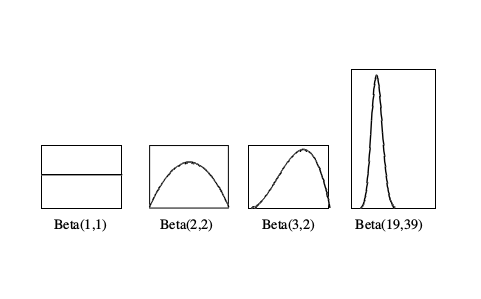
\includegraphics[scale=0.4]{figs/beta.png}
	\caption{几个beta分布}    
	\label{fig:beta}
\end{figure}


先验概率$p(\theta|\xi)$采用Beta分布有几个原因。首先,由公式\ref{eq:3},\marginpar{这里后验概率服从beta分布是如何推理的}\CJKunderwave*{可知后验概率$p(\theta|D,\xi)$也将服从beta分布}:
\begin{equation}
\label{eq:6}
p(\theta|D,\xi)
=\frac{\Gamma(\alpha+N)}{\Gamma(\alpha_h+h)\Gamma(\alpha_t+t)}\theta^{\alpha_h+h-1}(1-\theta)^{\alpha_t+t-1}
=Beta(\theta|\alpha_h+h,\alpha_t+t)
\end{equation}

其次,beta分布集是一个作为二项取样的共轭分布族。因此,这个分布中$\theta$的期望也有简单的形式:
\begin{equation}
\int \theta Beta(\theta|\alpha_h,\alpha_t)\, d\theta = \frac{\alpha_h}{\alpha}
\end{equation}
因此,我们很容易得出第N+1次抛掷图钉,针头朝上的概率的形式也简单,即
\begin{equation}
\label{eq:8}
p(X_{N+1}=heads|D,\xi)=\frac{\alpha_h+h}{\alpha+N}
\end{equation}


假定$p(\theta|\xi)$是beta分布,它可以评估多次。比如我们可以计算第一次抛掷图钉的概率(可以使用概率转盘)。第二步,我们可以想象已经看到了k次抛掷的结果,并且重新评估了下次抛掷时针头朝上的概率。对于等式\ref{eq:8}有:
\begin{equation}
p(X_1=heads|\xi)=\frac{\alpha_h}{\alpha_h+\alpha_t} \qquad
p(X_2=heads|X_1=heads,\xi)=\frac{\alpha_h+1}{\alpha_h+\alpha_t+1} \nonumber
\end{equation}
给定概率的表达式后,我们来解决$\alpha_h$和$\alpha_t$的取值问题。\marginpar{没有查到资料。。。}\CJKunderwave*{这种评估技术叫想象的未来数据。}


另外一种评估方法是基于公式\ref{eq:6}的。如果我们以先验$Beta(0,0)$\footnote{ 一般Beta的超参要取正数,这样可以标准化}开始,并且观察$\alpha_h$次针头朝上和$\alpha_t$次帽朝上,然后我们的后验概率(新的先验)满足$Beta(\alpha_h,\alpha_t)$分布。我们知道$Beta(0,0)$先验代表最小信息的情况,我们可以通过抛掷图钉针头和帽朝上的数目来评估$\alpha_h$和$\alpha_t$的值。或者,我们可以通过我们的当前经验来评估$p(X_1=heads|\xi)$和等同样本大小的$\alpha$,这个方法叫做\textbf{等价样本}。其他计算beta分布的方法Winkler(1967)、Chaloner和Duncan(1983)研究过。


虽然beta先验是方便的,但是对于一些问题是不准确的。比如,假设我们认为图钉可能是从魔法店买的。在这种情况下,合理的先验可能是混合beta分布。比如
\begin{equation}
p(\theta|\xi)=0.4 Beta(20,1) + 0.4 Beta(1,20) + 0.2 Beta(2,2) \nonumber
\end{equation}
其中0.4是图钉针头(帽)朝上的权重概率。实际上,我们已经介绍了一个隐藏变量$H$,它的值和三种情况有关:(1)图钉偏向头朝上,(2)图钉偏向帽朝上,(3)抛掷图钉,针头和帽朝上的可能性一样,并且假定每种情况都服从beta分布。通常有简单的方法(想象的未来数据法)来检测我们的信任是否是beta先验的正确反应。在那些beta先验不管用的情况下,通过引入额外的隐藏变量来进行评估不失为一个方法,就像上面的例子。


到目前为止,我们只是从二项分布来评估观察的结果。一般,观察结果可能是任何物理概率分布:
\begin{equation}
p(x|\boldsymbol{\theta},\xi)=f(x,\boldsymbol{\theta}) \nonumber
\end{equation}
其中$f(x,\boldsymbol{\theta})$是带有参数$\boldsymbol{\theta}$的似然函数\footnote{似然性是用于在已知某些观测所得到的结果时,对有关事物的性质的参数进行估计(而概率是用于在已知一些参数的情况下,预测接下来的观测所得到的结果)}。这里我们参数$\boldsymbol{\theta}$中参数个数是有限的。比如,$X$可能是连续变量,并且服从高斯分布$N(\mu,\nu)$:
\begin{equation}
p(x|\boldsymbol{\theta},\xi)=(2\pi \nu)^{-1/2}e^{-\frac{(x-\mu)^2}{2\nu}} \nonumber
\end{equation}
这里$\boldsymbol{\theta}={\mu,\nu}$。


不管函数是什么形式,在给定观察数据的前提下,我们都可以用贝叶斯方法来学习参数。就像我们在二项抽样的例中,我们定义那些变量和不知道的参数相关,引入先验概率,并且在给定观察数据的前提下,用贝叶斯规则来更新我们对这些参数的信任程度。
\begin{equation}
p(\boldsymbol{\theta}|D,\xi)=
\frac{p(D|\boldsymbol{\theta},\xi)p(\boldsymbol{\theta}|\xi)}{p(D|\xi)}
\end{equation}
然后我们对$\boldsymbol{\Theta}$所有的值取均值来作为下一次的预测值。比如
\begin{equation}
p(X_{N+1}=heads|D,\xi)
=\int p(X_{N+1}=heads|\theta,\xi)p(\theta|D,\xi)\, d\theta 
\end{equation}


对于指数族这类的分布,这些计算能以高效和相近的形式完成。指数族包括二项分布,多项式分布,正态分布,伽玛分布,泊松分布和多元正态分布。\marginpar{have sufficient statistics}\CJKunderwave*{指数族中每一个成员对固定维度的随机样本和简单的共轭先验有很大的统计意义}。


Bernardo和Smith(pp. 436-442,1994)总结了大量资料来使用指数族成员来进行贝叶斯计算。这里,我们总结了用于多项式抽样的这些项,并且提出了很多想法。


在多项式抽样中,观察的变量$X$是有r个可能取值$x^1,\cdots,x^r$的离散变量。似然函数如下:
\begin{equation}
p(X=x^k|\boldsymbol{\theta},\xi)=\theta_k,\, k=1,\cdots,r \nonumber
\end{equation}
其中$\boldsymbol{\theta}=\{\theta_2,\cdots,\theta_r\}$是参数($\theta_1=1-\sum_{k=2}^r \theta_k$)。
在这个例子里,参数是物理概率。而对数据集$D=\{X_1=x_1,\cdots,X_N=x_N\}$的有效统计是$\{N_1,\cdots,N_r\}$,$N_i$是在数据集D中$X=x^k$出现的次数。而用于多项式样本的共轭先验分布是狄利克雷分布\footnote{狄利克雷分布是一组连续多变量概率分布,是多变量普遍化的Β分布,常作为贝叶斯统计的先验概率。}。
\begin{equation}
p(\boldsymbol{\theta}|\xi)=Dir(\boldsymbol{\theta}|\alpha_1,\cdots,\alpha_r)=\frac{\Gamma(\alpha)}{\prod_{k=1}^r \Gamma(\alpha_k)}\prod_{k=1}^k \theta_k^{\alpha_k-1}
\end{equation}
其中$\alpha=\sum_{i=1}^r \alpha_k$,$\alpha_k>0,k=1,\cdots,r$。后验概率分布$p(\boldsymbol{\theta}|D,\xi)=Dir(\boldsymbol{\theta}|\alpha_1+N_1,\cdots,\alpha_r+N_r)$。包括想象的未来数据方法和等价样本法这些评估beta分布的方法也可以用来评估狄利克雷分布。在给定共轭先验概率和数据集D后,下一次观察结果的概率为
\begin{equation}
\label{eq:12}
p(X_{N+1}=x^k|D,\xi)=\int \theta_k Dir(\boldsymbol{\theta}|\alpha_1+N_1,\cdots,\alpha_r+N_r)\, d\boldsymbol{\theta}
=\frac{\alpha_k+N_k}{\alpha+N}
\end{equation}
而贝叶斯分析另一个重要的量是\marginpar{如何求取?}\textit{边缘似然}$p(D|\xi)$。在这种情况下,我们计算得出
\begin{equation}
\label{eq:13}
p(D|\xi)=\frac{\Gamma(\alpha)}{\Gamma(\alpha+N)}*\prod_{k=1}^r\frac{\Gamma(\alpha_k+N_k)}{\Gamma(\alpha_k)}
\end{equation}


我们注意到公式里提交的知识$\xi$是有用的,因为它强调了概率是主观的。然而,一旦这个观念牢固,这样的表示就会有点麻烦。所以在这篇论文的后面部分,我们就不显式的提及$\xi$了。


在这部分的最后,我们强调了一点,就是虽然贝叶斯方法和古典方法有时能得到相同的预测,但是它们对于从数据中学习是完全不同的方法。现在我们重新审视一下图钉的问题。求解图钉针头朝上概率的贝叶斯方法和古典方法是完全相反的。


在古典方法中,$\theta$是固定的(虽然不知道是多少),并且想象所有的数据集可能来自由$\theta$决定的二项分布中抽样生成。每个数据集发生的概率是$p(D|\theta)$并且将会产生一个估计值$\theta*(D)$。为了评估这个估计值,我们计算所有这样的数据集的期望和方差。
\begin{eqnarray}
\label{eq:14}
E_{p(D|\theta)}(\theta^*)&=&\sum_D p(D|\theta) \theta^*(D) \nonumber \\
Var_{p(D|\theta)}(\theta^*)&=&\sum_D p(D|\theta) (\theta^*(D)-E_{p(D|\theta)}(\theta^*))^2
\end{eqnarray}


我们选择一个估计值来均衡估计值和$\theta$的偏差$(\theta-E_{p(D|\theta)}(\theta^*))$和方差\footnote{低偏差和方差不只是评估值想要的属性,像一致性和撸棒性也是。}。最后,我们用这个评估值来评估我们观察到的数据集。一般采用的评估法是最大似然(ML)方法--选择某个$\theta$来使边缘似然$p(D|\theta)$最大化。对于二项取样,我们有
\begin{equation}
\theta_{ML}^*(D)=\frac{N_k}{\sum_{k=1}^r N_k} \nonumber
\end{equation}


对于这样(或其他类型)的取样,最大似然估计(ML)是无偏的。也就是说对于$\theta$的所有值,ML是没有误差。此外,对于$\theta$的所有值,ML评估法的方差是比其他任何无偏估计法要小(Schervish,1995)。

相反,在贝叶斯方法中,数据集D是固定的,并且假定这个数据集中所有$\theta$可能的值能够生成。给定$\theta$,图钉针头朝上的物理概率就是$\theta$它本身。然而,$\theta$不确定,所以我们最终的评估是我们后验概率$\theta$的期望。
\begin{equation}
\label{eq:15}
E_{p(\theta|D,\xi)}(\theta)=\int\theta p(\theta|D,\xi)\, d\theta
\end{equation}


公式\ref{eq:14}和\ref{eq:15}中的期望是不同的,这将导致不同的评估。构成差异一种说法是古典方法和贝叶斯方法对好的评估有不同的定义。两个结果都是“正确”的,也就是说它们是一致的。不幸的是两种方法都有它们的缺点,这也导致了每种方法的优点被诟病。比如,支持贝叶斯的人说不理解公式\ref{eq:14}中的期望,因为我们只看到一个单个数据集。如果我们能够得到更多的数据集,我们可以把它们合并成一个更大的数据集。相反,支持古典方法的统计学者认为在许多情况足够正确的先验是不容易估计的。一般的观点是使用对手头任务最敏感。不过我们认为贝叶斯方法已经在使用,特别是根据前言中提及的优势。在这篇文章中,我们聚焦在贝叶斯方法上。


\section{贝叶斯网络}
到目前为止,我们只考虑带有一个或少量变量的简单问题。然而在真正的学习问题中,我们感兴趣的是探寻大量变量之间的关系。贝叶斯网络是适合这个任务的代表。它是一个图模型,能够有效的描述大量变量集的联合概率分布。在这部分,我们定义了贝叶斯网络并且介绍了如何从先验知识构建贝叶斯网络。


包含变量集$\boldsymbol{X}=\{X_1,\cdots,X_n\}$的贝叶斯网络包含一个描述变量集$\boldsymbol{X}$中变量间条件独立的网络结构和与每个变量相关条件概率分布集P。这两部分定义了$\boldsymbol{X}$的联合概率分布。网络结构S是个有向无环图。S中的一个节点代表$\boldsymbol{X}$中的一个变量。我们用$X_i$代表变量和它相关的节点,而$\boldsymbol{Pa}_i$代表网络结构S中$X_i$的父节点集。而S中可能缺失的弧代表是否条件独立。特别的,给定结构S,$\boldsymbol{X}$的联合概率是
\begin{equation}
\label{eq:16}
p(x)=\prod_{i=1}^n p(x_i|pa_i)
\end{equation}
概率分布P是和公式\ref{eq:16}相关的项。(S,P)能描述联合分布$p(x)$。


贝叶斯网络中的概率可能是物理概率也可能是贝叶斯概率。当只从先验概率学习贝叶斯网络是,用的是贝叶斯概率。当从数据中学习贝叶斯网络时,用的是物理概率(他们的值可能不确定)。在子部分,我们将介绍如何从数据中学习贝叶斯网络的结构和概率。在后面的部分,我们探究从先验知识构建贝叶斯网络。在第十部分,这个过程对于贝叶斯网络也是很有帮助的。


为举例说明构建贝叶斯玩过的过程,考虑检验信用卡欺骗的问题。首先来确定这个模型的变量。其中一组可能的变量是Fraud(F),Gas(G),Jewelry(J),Age(A)和Sex(S):Fraud表示当前的购买是否是欺骗的,Gas表示在最近的24小时是否有天然气交易,Jewelry表示在最近的24小时是否有珠宝交易,Age和Sex表示持卡者的年龄和性别。变量间的关系如图\ref{fig:structure}所示。当然,在现实问题中,我们会包含更多的变量。同样,\marginpar{model the states of one or more of these variables at a finer level of detail.}\CJKunderwave*{我们也可以对一个或多个变量的状态以更好的细节水平建模}。比如,我们可以设置Age为连续变量。
\begin{figure}[!htbp]
	\centering
    	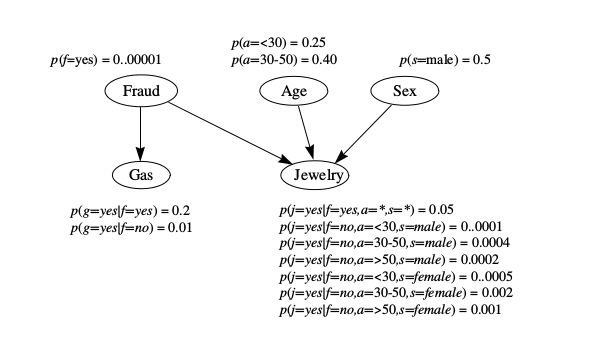
\includegraphics[scale=0.4]{figs/structure.png}
	\caption{检测信用卡欺骗的贝叶斯网络:弧是由因指向果。和节点相关的概率分布是和邻近节点相关的。星号代表任意状态。}    
	\label{fig:structure}
\end{figure}

问题的解决不是一步到位的。首先,我们必须(1)正确识别模型的目的(比如说预测,解释和探究),(2)识别许多可能和问题相关的观察值,(3)决定这些观察值的哪些子集是值得建模的,(4)将观察值赋值给相互独立完全穷尽\footnote{相互独立是指事件间两两独立,完全穷尽是指所有事件发生的可能性之和为1}的变量。这里的困难不是建立唯一的贝叶斯网络,但是大部分方法是一般的。虽然没有明确的解决方案,但是一些决策分析师(Howard and Matheson,1983)和统计学家(Tukey,1977)还是提供了一些指南。


在贝叶斯网络构建的下个阶段,我们构建一个有向无环图来表示条件独立性的断言。这样做的方法是基于下面的观察。根据概率的链式规则,我们有
\begin{equation}
\label{eq:17}
p(x)=\prod_{i=1}^n p(x_i|x_1,\cdots,x_{i-1})
\end{equation}
对于每个$X_i$,有些子集$\Pi_i \in \{X_1,\cdots,X_{i-1}\}$能保证$X_i$和$\{X_1,\cdots,X_{i-1}\} \backslash \Pi_i$是条件独立的。也就是说,对于任何x,
\begin{equation}
\label{eq:18}
p(x_i|x_1,\cdots,x_{i-1})=p(x_i|\pi_i)
\end{equation}
结合公式\ref{eq:17}和公式\ref{eq:18},可以得到
\begin{equation}
\label{eq:19}
p(x)=\prod_{i=1}^n p(x_i|\pi_i)
\end{equation}


相比较公式\ref{eq:16}和\ref{eq:19},变量集$(\Pi_1,\cdots,\Pi_n)$等价于贝叶斯网络的父节点$(\boldsymbol{Pa}_1,\cdots,\boldsymbol{Pa}_n)$。在网络结构中它们依次指明了弧。


为确定贝叶斯网络的结构,我们首先将变量排序,然后确定像公式\ref{eq:18}中的变量集。在我们这个例子里,使用顺序(F,A,S,G,J),并有如下的条件独立
\begin{eqnarray}
p(a|f)&=&p(a) \nonumber \\
p(s|f,a)&=&p(s) \nonumber \\
p(g|f,a,s)&=&p(g|f) \nonumber \\
p(j|f,a,s,g)&=&p(j|f,a,s)
\label{eq:20}
\end{eqnarray}
因此,我们得到了图\ref{fig:structure}的结构。


这个方法有严重的缺点。如果我们粗心地选择变量顺序,那么最终的网络结构可能不能揭示许多变量间的条件独立性。比如,如果我们用(J,G,S,A,F)顺序来构建贝叶斯网络,我们将会得到一个完全连通的网络结构。因此,最坏的情况是我们将会探究$n!$个变量顺序来找出最好的一个。幸运的是,有另外一种方法可以不需要顺序来构建贝叶斯网络。这种方法是基于两点观察:(1)人们通常能迅速的判断出变量间的因果关系,(2)因果关系等价于条件独立的断言。特别的,要将一个变量集构建成贝叶斯网络,只要从因变量画个弧到果变量。在几乎所有的情况下,这样做所构成的网络结构是满足公式\ref{eq:16}的定义的。比如,断言信用卡欺骗是汽油交易的直接原因,信用卡欺骗,年龄和性别是珠宝交易的直接起因,我们也可以获得图\ref{fig:structure}这个哦你的网络结构。贝叶斯网络中的因果关系很大程度保证了贝叶斯网络能够作为一个专家系统(Heckerman,1995)的代表。在第15部分,我们简爱嗯会看到如果使用因果语义来从数据中学习因果关系。


构建贝叶斯网络的最后一步是计算条件概率分布$p(x_i|\boldsymbol{pa}_i)$.在信用卡欺骗的例子里,所有变量是离散型的,我们可以计算$X_i$在$\boldsymbol{Pa}_i$中每个变量下的条件概率。具体的例子见图\ref{fig:structure}。


虽然我们描述了构建网络的一系列步骤,但是在实际中他们经常是混乱的。比如,条件独立性或因果关系的判断会影响问题。同样,条件概率分布的计算也能导致网络结构的改变。在Jensen(1996)的文中可以发现例子来熟悉贝叶斯网络的构建过程。


\section{贝叶斯网络中的推理}
一旦我们从先验知识,数据或者二者构建贝叶斯网络,我们通常需要从这个模型中获得各种感兴趣的概率。比如,在欺骗检验的例子中,我们想要知道在给定其他变量的观察值的前提下,信用卡欺骗的概率是多少。这个概率不是直接存储在模型中的,因此需要计算。一般,计算给定模型中感兴趣事件的概率叫做概率推理。这部分将介绍贝叶斯网络中的概率推理。


由变量集$\boldsymbol{X}$构建的贝叶斯网络决定了$\boldsymbol{X}$的联合概率分布,原则上,我们可以用贝叶斯网络来计算任何感兴趣事件的概率。比如说,图\ref{fig:structure}中的贝叶斯网络,在给定其他变量的观察值下信用卡欺骗的概率是
\begin{equation}
p(f|a,s,g,j)=\frac{p(f,a,s,g,j)}{p(a,s,g,j)}=\frac{p(f,a,s,g,j)}{\sum_{f'} p(f',a,s,g,j)}
\label{eq:21}
\end{equation}
然而,对于有很多变量的问题,这种直接的方法不实用。幸运的是,当所有的变量是离散型时,我们可以探究贝叶斯网络中的条件独立来使计算更高效。在本文的例子里,在给定如公式\ref{eq:20}中的条件独立,公式\ref{eq:21}就变成
\begin{eqnarray}
p(f|a,s,g,j)&=&\frac{p(f)p(a)p(g|f)p(j|f,a,s)}{\sum_{f'} p(f')p(a)p(s)p(g|f')p(j|f‘,a,s)} \\
&=&\frac{p(f)p(g|f)p(j|f,a,s)}{\sum_{f'} p(f')p(g|f')p(j|f‘,a,s)} \nonumber 
\end{eqnarray}


研究人员已经研究出贝叶斯网络的概率推理算法,不过该算法只能粗略的探究条件独立的离散变量。比如,\marginpar{这里很多论文可以看看}Howard和Matheson(1981),Olmsted(1983)和Shachter(1988)研究出一种算法,它通过反转网络中弧的方向知道给定概率查询的结果能够直接从图模型中直接读出来。其中,每个弧的反转代表一次贝叶斯理论的应用。Pearl(1986)开发出了消息传递模型,通过一个或多个变量的观察值来更新贝叶斯网络中每个节点的概率分布。Lauritzen和Spiegelhalter(1988),Jensen(1990)和Dawid(1992)研究了一个算法。它先将贝叶斯网络转换成树,树中的每个节点等价于$\boldsymbol{X}$中变量的子集。然后,算法用树里的数学属性来进行概率的推理。最近,D’Ambrosio(1991)研究出一个推理算法来简化公式\ref{eq:21}和公式\ref{eq:22}中的和与积。最常用的处理离散变量贝叶斯网络的算法是Lauritzen和Spiegelhalter(1988),Jensen(1990)和Dawid(1992)。


Shachter和Kenley(1989)和Lauritzen(1992)发现了一个方法用来对多变量的高斯分布或混合高斯分布的贝叶斯网络进行精确推理。这些方法也使用条件独立性来简化推理。对于包含其他分布的贝叶斯网络中的推理方法,比如一般的线性回归模型也被研究出来(Saul,1996;jaakkola和jordan,1996)。


虽然我们使用条件独立来简化概率推理,但是包含离散变量的任意贝叶斯网络中的推理是个NP难题(Cooper,1990)。甚至大概的推理(比如Monte-Carlo方法)也是NP难题(Dagum和Luby,1993)。难点在于贝叶斯网络结构中的无向环(忽视贝叶斯网络结构中弧的方向)。(如果我们在图\ref{fig:structure}中添加一个从Age到Gas的弧,就会获得一个无向环:F-G-A-J-F。)当贝叶斯网络结构包含许多无向环,推理就变得棘手。然而,对于许多应用,结构要足够的简单才能使推理更高效。对于某些应用,一般的推理方法是不实际的,研究者正在研究一般的方法来适用特别的拓扑网络结构(Heckerman,1989; Suermondt and Cooper, 1991; Saul, 1996; Jaakkola and
Jordan, 1996)和特别的推理查询(Ramamurthi and Agogino, 1988; Shachter, 1990; Jensen and Andersen, 1990; Darwiche and Provan, 1996)。


\section{贝叶斯网络中的概率学习}
在下面的几个部分,我们将展示如何从给定的数据中提取出贝叶斯网络的结构和概率分布。结论就是很多数据分析的技术,它们结合先验知识和数据来产生更优良的知识。在这个部分,我们考虑最简单的问题版本:用数据来更新给定贝叶斯网络结构的条件概率表。


回忆一下,在图钉的问题中,我们没有学习图钉针头朝上的概率。相反,我们对代表针头朝上概率这个变量的后验概率进行更新。在贝叶斯网络中我们采用相同的方法来处理概率。特别的,我们假定变量集$\boldsymbol{X}$的联合概率分布可以被一些网络结构S所描述。
\begin{equation}
p(\boldsymbol{x}|\boldsymbol{\theta}_s,S^h)=\prod_{i=1}^n p(x_i|\boldsymbol{pa}_i,\boldsymbol{\theta}_i,S^h)
\end{equation}
其中$\boldsymbol{\theta}_i$是分布$p(x_i|\boldsymbol{pa}_i,\boldsymbol{\theta}_i,S^h)$的参数向量,$\boldsymbol{\theta}_s$是参数矩阵$\{\boldsymbol{\theta}_1,\cdots,\boldsymbol{\theta}_n\}$,$S^h$代表联合概率分布可以被结构S\footnote{网络结构的假设重叠。比如,给定变量集$\boldsymbol{X}=\{X_1,X_2\}$,$\boldsymbol{X}$的概率分布包含了无弧的网络结构和$X_1->X_2$的网络结构。 这个重叠代表模型平均的问题,并将在第七部分描述。因此,我们可以在定义中添加条件来确保无重复。Heckerman和Geiger(1996)描述了这个条件集。}包含在内这事件(统计学里术语叫“假说”)。此外,我们假定从联合概率分布中获得了随机样本$D=\{x_1,\cdots,x_N\}$。我们以D中的元素$x_l$为例。正如第二部分,我们通过定义(向量)变量$\Theta_s$来描述参数$\boldsymbol{\theta}_s$的不确定性,并且评估先验概率密度函数$p(\boldsymbol{\theta}_s|S^h)$。在贝叶斯网络里学习概率的问题可以简化为:给定一个随机样本D,计算后验概率$p(\boldsymbol{\theta}_s|D,S^h)$。


我们把分布$p(x_i|\boldsymbol{pa}_i,\boldsymbol{\theta}_i,S^h)$(关于$\boldsymbol{\theta}_i$的函数)叫做局部分布函数。熟悉监督学习的读者会意识到分布函数不过是一个概率分类或回归函数。因此,贝叶斯网络可以看作以条件独立关系建立的概率分类/回归模型的集合。产生概率结果的分类/回归模型有线性回归,一般的线性回归,神经网络(MacKay,1992a,1992b),决策树(Buntine,1993;Friedman和Goldszmidt,1996),核密度评估方法(Book,1994)和字典方法(Friedman,1995)。原则上,上述任意一种方法都可以用来学习贝叶斯网络里的概率;在大部分情况,贝叶斯学习方法是容易获得的。然而,大部分学习模型都包括无约束的多项式分布(Cooper和Herskovits,1992),包含高斯噪声的线性回归(Buntine,1994;Heckerman和Geiger,1996)和一般的线性回归(MacKay,1992a和1992b;Neal,1993;Saul,1996)。


在本文中,我们使用无限制的多项式分布来介绍概率学习的基本方法。这里,每个变量$X_i \in \boldsymbol{X}$是离散的,有$r_i$个可能的值$x_i^1,\cdots,x_i^{r_i}$,每个局部分布函数是多项式分布的集合,一个分布代表一个$\boldsymbol{Pa}_i$的配置。所以我们假定
\begin{equation}
\label{eq:24}
p(x_i^k|\boldsymbol{pa}_i^j,\boldsymbol{\theta}_i,S^h)=\theta_{ijk} >0
\end{equation}
这里$\boldsymbol{Pa}_i^1,\cdots,\boldsymbol{Pa}_i^{q_i}(q_i=\prod_{X_i \in \boldsymbol{Pa}_i} r_i)$代表$\boldsymbol{Pa}_i$的配置,$\boldsymbol{\theta}_i=((\theta_{ijk})_{k=2}^{r_i})_{j=1}^{q_i}$是个参数矩阵(参数$\theta_{ij1}=1-\sum_{k=2}^{r_i}\theta_{ijk}$).方便起见,对于所有的i和j,我们定义参数向量
\begin{equation}
\boldsymbol{\theta}_{ij}=(\theta_{ij2},\cdots,\theta_{ijr_i})	\nonumber
\end{equation}
我们使用术语“非限制”来对比这个分布和拥有$\boldsymbol{Pa}_i$低维函数的多项式分布--比如说一般线性回归模型。


\begin{quotation}
这段里面说得并不是很清楚,特别是关于$\boldsymbol{Pa}_i$的配置。这里以图\ref{fig:structure}中的Fraud(F),Age(A),Sex(S)和Jewelry(J)的四个变量来说明。由图易知Jewelry的父节点有Fraud,Age和Sex。其中$p(Fraud=x_1^1)=0.00001,p(Fraud=x_1^2)=0.9999;p(Age=x_2^1)=0.25,p(Age=x_2^2)=0.4,p(Age=x_2^3)=0.35;p(Sex=x_3^1)=0.5,p(Sex=x_3^2)=0.5$)而对于变量Jewelry我们可以获得如下的概率分布表
\begin{table}[!hbp]%开始表格
\caption{Jewelry的概率分布表} %表格的名称
\label{tab:local probility}
\begin{center}
\begin{tabular}{c c c | c c}%开始绘制表格
\hline %绘制一条水平的线
Fraud	&	Age	&	Sex	&	Jewelry	&	$\overline{Jewelry}$\\
\hline
$x_1^1$		&	$x_2^1$	&	$x_3^1$	&	0.05		&	0.95		\\
$x_1^1$		&	$x_2^1$	&	$x_3^2$	&	0.05		&	0.95		\\
$x_1^1$		&	$x_2^2$	&	$x_3^1$	&	0.05		&	0.95		\\
$x_1^1$		&	$x_2^2$	&	$x_3^2$	&	0.05		&	0.95		\\
$x_1^1$		&	$x_2^3$	&	$x_3^1$	&	0.05		&	0.95		\\
$x_1^1$		&	$x_2^3$	&	$x_3^2$	&	0.05		&	0.95		\\
$x_1^2$		&	$x_2^1$	&	$x_3^1$	&	0.0001	&	0.9999	\\
$x_1^2$		&	$x_2^1$	&	$x_3^2$	&	0.0005	&	0.9995	\\
$x_1^2$		&	$x_2^2$	&	$x_3^1$	&	0.0004	&	0.9996	\\
$x_1^2$		&	$x_2^2$	&	$x_3^2$	&	0.002	&	0.998	\\
$x_1^2$		&	$x_2^3$	&	$x_3^1$	&	0.0002	&	0.9998	\\
$x_1^2$		&	$x_2^3$	&	$x_3^2$	&	0.001	&	0.999	\\
\hline
\end{tabular}
\end{center}
\end{table}
结合表\ref{tab:local probility}看公式\ref{eq:24},其中$x_i^k$表示Jewelry这个变量的第k个取值(状态),$\boldsymbol{Pa}_i$表示Jewelry的父节点集,而它的配置就是表格中的每一行,所以$\boldsymbol{Pa}_i^j$表示父节点集的第j个配置,共有$q_i=\prod_{X_i \in \boldsymbol{Pa}_i} r_i$个配置。$\boldsymbol{\theta}_i$就表示表中的概率矩阵。而$\boldsymbol{\theta}_{ij}$表示Jewelry变量在父节点集下的第j个配置的概率分布。其和相加为1,对应表格中就是每一行。
\end{quotation}


在给定这类局部分布函数的情况下,我们能够快速的计算后验概率$p(\boldsymbol{\theta}_s|D,S^h)$。当然这要基于两个假设前提,第一个是在随机样本D中没有丢失数据,换句话说随机样本是完整的。第二个是参数向量$\boldsymbol{\theta}_{ij}$是相互独立的。也就是说
\begin{equation}
p(\boldsymbol{\theta}_s|S^h)=\prod_{i=1}^n\prod_{j=1}^{q_i}p(\boldsymbol{\theta}_{ij}|S^h) 
\end{equation}
第二个假设叫参数独立,Spiegelhalter和Lauritzen(1990)介绍了这一假设。


因此,我们可以独立的更新每一个参数向量$\boldsymbol{\theta}_{ij}$,就像在一个变量的例子里。假设,每个向量$\boldsymbol{\theta}_{ij}$服从先验分布$Dir(\boldsymbol{\theta}_{ij}|\alpha_{ij1},\cdots,\alpha_{ijr_i})$,我们可以得到后验分布
\begin{equation}
p(\boldsymbol{\theta}_{ij}|D,S^h)=Dir(\boldsymbol{\theta}_{ij}|\alpha_{ij1}+N_{ij1},\cdots,\alpha_{ijr_i}+N_{ijr_i})
\end{equation}
其中$N_{ijk}$是D中$X_i=x_i^k,\boldsymbol{Pa}_i=\boldsymbol{pa}_i^j$这种情况出现的次数。


在图钉的例子中,我们可以用$\boldsymbol{\theta}_s$可能值的平均来表示下次的预测。这里,我们来计算$p(\boldsymbol{x}_{N+1}|D,S^h)$,$\boldsymbol{x_{N+1}}$是获得数据集D后下一次所看到的结果。假定,在第N+1次结果中,$X_i=x_i^k,\boldsymbol{Pa}_i=\boldsymbol{pa}_i^j$,其中k和j依赖于i。因此
\begin{equation}
p(\boldsymbol{x}_{N+1}|D,S^h)=E_{p(\boldsymbol{\theta}_s|D,S^h)}(\prod_{i=1}^n\theta_{ijk})  \nonumber
\end{equation}
为了计算这个期望,我们首先根据参数向量相互独立这个假设:
\begin{equation}
p(\boldsymbol{x}_{N+1}|D,S^h)=\int \prod_{i=1}^n \theta_{ijk} p(\boldsymbol{\theta}_s|D,S^h)\, d\boldsymbol{\theta}_s
=\prod_{i=1}^n \int \theta_{ijk}p(\boldsymbol{\theta}_{ij}|D,S^h)\,d\boldsymbol{\theta}_{ij} \nonumber
\end{equation}
由公式\ref{eq:12},上式就变成
\begin{equation}
\label{eq:27}
p(\boldsymbol{x}_{N+1}|D,S^h)=\prod_{i=1}^n \frac{\alpha_{ijk}+N_{ijk}}{\alpha_{ij}+N_{ij}}
\end{equation}
其中$\alpha_{ij}=\sum_{k=1}^{r_i}\alpha_{ijk},N_{ij}=\sum_{k=1}^{r_i}N_{ijk}$。
这些计算是简单的,因为非限制的二项式分布是指数簇家族。对于高斯噪声线性回归的计算也是直接的(Buntine,1994;Heckerman and Geiger,1996)。


\begin{quotation}
这部分是将图钉样例中的推理方法使用到贝叶斯网络中。这里,我们只知道网络结构和样本集D,要求得是每个节点的局部概率分布。本文作者先假设表\ref{tab:local probility}中每一行都服从先验分布$Dir(\boldsymbol{\theta}_{ij}|\alpha_{ij1},\cdots,\alpha_{ijr_i})$,并通过样本集D来预测下一次某个事件发生的概率。比如
\begin{eqnarray}
p(Fraud=x_1^1,Age=x_2^1,Sex=x_3^1,Gas=x_5^1,Jewelry=x_4^1) \nonumber\\
=p(x_1^1)*p(x_2^1)*p(x_3^1)p(x_5^1|x_1^1)*p(x_4^1|x_1^1,x_2^1,x_3^1) \nonumber\\
=\theta_{111}*\theta{211}*\theta_{311}*\theta_{511}*\theta_{411}
\nonumber
\end{eqnarray}
这就是为嘛计算期望的公式中变量会是$\prod_{i=1}^n\theta_{ijk}$,这里$p(\boldsymbol{\theta}_s|D,S^h)$是指已知网络结构和数据集D的前提下,所有的节点的局部概率分布为$\boldsymbol{\theta}_s$的概率。当$\boldsymbol{\theta}_s$一定时,根据$\prod_{i=1}^n\theta_{ijk}$很容易求出某个事件发生的概率。最后因为非限制的二项式分布是指数簇家族的一员,可以直接求出期望。简化了计算。
\end{quotation}



\section{处理不完整数据的方法}
现在我们再来讨论一下当随机样本是不完整(在某些情况下一些变量无法获取观察值)时如何进行贝叶斯网络的参数学习。\marginpar{翻译有问题}\CJKunderwave*{它与丢失数据的重要区别在于缺失的观察值是否依赖变量的实际状态}。比如,在药物学习中,缺失的数据可能意味着病人太虚弱以至无法进行研究,虚弱的原因可能是药物的副作用。相反,如果变量是隐藏的(在任何情况下都没有去观察),则这个数据的缺失是独立于这个状态的。虽然贝叶斯方法和图模型适合分析这两种情况,但是处理那些丢失的独立与状态的数据比那些依赖于状态的数据更简单。在本文中,我们只考虑简单的情况。对复杂的情况感兴趣的读者可以看Rubin(1978),Robins(1986)和Pearl(1995)。


继续我们使用非限制二项式分布的例子,假定我们看到一个数据不完全的样例。$\boldsymbol{Y} \in \boldsymbol{X}$代表例中可以观察的变量集,而$\boldsymbol{Z} \in \boldsymbol{X}$代表例中不可以观察的变量集。在参数独立的假定下,我们可以计算网络结构S中$\boldsymbol{\theta}_{ij}$的后验概率为

\begin{eqnarray}
\label{eq:28}
p(\boldsymbol{\theta}_{ij}|\boldsymbol{y},S^h)&=&
\sum_{\boldsymbol{z}} p(\boldsymbol{z}|\boldsymbol{y},S^h)p(\boldsymbol{\theta_{ij}}|\boldsymbol{y},\boldsymbol{z},S^h)\\
&=&(1-p(\boldsymbol{pa}_i^j|\boldsymbol{y},S^h))\{p(\boldsymbol{\theta}_{ij}|S^h)\}+
\sum_{k=1}^{r_i}p(x_i^k,\boldsymbol{pa}_i^j|\boldsymbol{y},S^h)\{p(\boldsymbol{\theta}_{ij}|x_i^j,\boldsymbol{pa}_i^j,S^h)\}\nonumber
\end{eqnarray}
详情见Spiegelhalter and Lauritzen(1990)。公式\ref{eq:28}中大括号中的项服从狄利克雷分布。除非$\boldsymbol{X}_i$和$\boldsymbol{Pa}_i$中的所有变量都在$\boldsymbol{y}$中可观察。不然$\boldsymbol{\theta}_{ij}$的后验概率就是狄利克雷分布的线性组合,换句话说,是狄利克雷函数和参数$(1-p(\boldsymbol{pa}_i^j|\boldsymbol{y},S^h)),p(x_i^k,\boldsymbol{pa}_i^j|\boldsymbol{y},S^h),k=1,\cdots,r_i$的组合。


\subsection{Monte-Carlo方法}
评估的一种方法是基于Monte-Carlo\footnote{Monte-Carlo算法,又称随机模拟法/统计实验方法。它泛指一类算法,在这些算法中,要求解的问题是某随机事件的概率或某随机变量的期望。这时,通过“实验”方法,用频率代替概率或得到随机变量的某些数字特征,以此作为问题的解。}或随机样本方法。当花费足够长时间来计算聚合,那么这种评估是正确的。


这部分,我们来讨论众多Monte-Carlo方法中的一种,叫吉布斯采样,是由Geman和Geamn(1984)中详细描述。给定有着相同的联合概率$p(x)$的变量集$\boldsymbol{X}=\{X_1,\cdots,X_n\}$,我们用吉布斯样本发生器来评估函数$f
(x)$的期望。首先,我们确定变量集$\boldsymbol{X}$中每个变量的初始状态(随机生成)。然后,我们挑选其中一个(一些)变量$X_i$(不赋予当前的值),并通过其他n-1个变量来推算它的概率分布。接着,基于这个概率分布,我们抽取$X_i$的状态,并计算$f(x)$,最终我们遍历先前的两步,并求取$f(x)$的均值。当样例的数目达到无穷时,所求的均值就等价于$E_{p(x)}(f(x))$。首先,吉布斯样本发生器必须是不可减的(irreducible)。概率分布$p(x)$必须能够抽取$\boldsymbol{X}$中任何配置。比如,如果$p(x)$不包括零概率,那么吉布斯样本发生器将会是不可减的。其次,每个$X_i$必须有有限的状态。实际上,通过移动变量的算法通常被采用。关于吉布斯取样和其他Monte-Carlo方法包括初始化方法和收敛的讨论将会在Neal(1993)和Madigan and York(1995)。


下面举例说明吉布斯采样,首先在给定不完全数据集$D=\{y_1,\cdots,y_N\}$和由服从独立狄利克雷先验的离散变量构成的贝叶斯网络下,我们假设一些$\boldsymbol{\theta}_s$的配置的概率密度为$p(\boldsymbol{\theta}|D,S^h)$。为估算$p(\boldsymbol{\theta}|D,S^h)$,我们首先初始化每种情况中无法观察变量的状态。因此我们获得一个完全的随机样本$D_c$,接着,我们选择一些在原先随机样本$D$中没有被观察的变量$X_{il}$(变量$X_i$在第l个样例),并根据下面的概率分布重新赋值
\begin{equation}
p(x_{il}^{'}|D_c\backslash x_{il},S^h)=
\frac{p(x_{il}^{'},D_c\backslash x_{il}|S^h)}
{\sum_{x_{il}^{'}} p(x_{il}^{''},D_c\backslash x_{il}|S^h)} \nonumber
\end{equation}
其中,$D_c\backslash x_{il}$表示去掉观察值$x_{il}$后的数据集$D_c$,分母上的和是指变量$X_{il}$所有的状态。就想我们在第七部分所见,分子和分母中的项是可以快速计算(见公式\ref{eq:35}).然后,我们对$D$中所有的没有观察的变量重复这个再赋值过程,直到产生一个新的完整的随机样本$D_c^{'}$。最后,我们遍历先前的三个步骤并使用$p(\boldsymbol{\theta}|D_c^{'},S^h)$的均值来作为评估的结果。


\subsection{高斯评估}
Monte-Carlo方法产生精确的结果,但是他们通常难以处理,特别是当样本大小很大时。另一个比Monte-Carlo方法更高效的评估方法是高斯评估(Kass etal。1988;kass and raftery,1995),特别是很大的样本。


对于大量的数据,$p(\boldsymbol{\theta}_s|D,S^h) \propto p(D|\boldsymbol{\theta}_s,S^h)*p(\boldsymbol{\theta}_s|S^h)$通常被当作混合高斯分布来评估。特别的,
\begin{equation}
\label{eq:29}
g(\boldsymbol{\theta}_s)\equiv \log(p(D|\boldsymbol{\theta}_s,S^h)*p(\boldsymbol{\theta}_s|S^h))
\end{equation}
定义使$g(\boldsymbol{\theta}_s)$最大时的$\boldsymbol{\theta}_s$为$\overline{\boldsymbol{\theta}}_s$。该配置$\overline{\boldsymbol{\theta}}_s$同样会使$p(\boldsymbol{\theta}_s|D,S^h)$取得最大值,这也叫做$\boldsymbol{\theta}_s$的最大的后验配置(MAP)。使用关于$\overline{\boldsymbol{\theta}}_s$的$g(\boldsymbol{\theta}_s)$的二次泰勒多项式来评估$g(\boldsymbol{\theta}_s)$。我们获得
\begin{equation}
\label{eq:30}
g(\boldsymbol{\theta}_s) \approx g(\overline{\boldsymbol{\theta}}_s)-\frac{1}{2}
(\boldsymbol{\theta}_s-\overline{\boldsymbol{\theta}}_s)A
(\boldsymbol{\theta}_s-\overline{\boldsymbol{\theta}}_s)^t
\end{equation}
其中$(\boldsymbol{\theta}_s-\overline{\boldsymbol{\theta}}_s)^t$是行向量$(\boldsymbol{\theta}_s-\overline{\boldsymbol{\theta}}_s)$的转置。A是$g(\boldsymbol{\theta}_s)$的非负海瑟矩阵\footnote{海瑟矩阵是一个自变量为向量的实值函数的二阶偏导数组成的方块矩阵}。将上式代入到公式\ref{eq:29}中可得
\begin{eqnarray}
\label{eq:31}
p(\boldsymbol{\theta}_s|D,S^h) &\propto & 
p(D|\boldsymbol{\theta}_s,S^h)*p(\boldsymbol{\theta}_s|S^h)\\
& \approx & p(D|\overline{\boldsymbol{\theta}}_s,S^h)*p(\overline{\boldsymbol{\theta}}_s|S^h)\exp\{-\frac{1}{2}
(\boldsymbol{\theta}_s-\overline{\boldsymbol{\theta}}_s)A
(\boldsymbol{\theta}_s-\overline{\boldsymbol{\theta}}_s)^t\}\nonumber
\end{eqnarray}
因此,$p(\boldsymbol{\theta}_s|D,S^h)$差不多服从高斯分布。

为计算高斯评估值,我们必须计算$\overline{\boldsymbol{\theta}}_s$和非负海瑟矩阵A。在下面部分,我们来讨论方法来求解$\overline{\boldsymbol{\theta}}_s$。Meng和Rubin(1991)描述了一个数值方法来计算二次求导。Raftery(1995)描述了用似然率方法(在统计学中常用)来评估海瑟矩阵。Thiesson(1995)证明了对于非限制的多维分布,二次导数可以用贝叶斯网络的推理来计算。



\subsection{MAP及ML评估和EM算法}
随着数据样本大小的增加,高斯峰值将会变得更尖,趋向于MAP配置$\overline{\boldsymbol{\theta}}_s$中的$\delta$函数。在这个限制下,我们没有必要去计算均值或期望。相反,我们只要基于MAP配置作出预测就好。


更进一步的估算是基于下面的观察,即当样本大小增加是,先验$p(\boldsymbol{\theta}_s|S^h)$的影响就下降了。因此我们通过求$\boldsymbol{\theta}_s$配置的最大似然来评估$\overline{\boldsymbol{\theta}}_s$:
\begin{equation}
\overline{\boldsymbol{\theta}}_s=\arg \max_{\boldsymbol{\theta}_s} \{p(D|\boldsymbol{\theta}_s,S^h)\} \nonumber
\end{equation}


求解ML或MAP的一种方法是基于梯度的优化。比如,我们使用梯度递增来使$g(\boldsymbol{\theta}_s)$的导数达到局部最大。Russell et al。(1995)and Thiesson(1995)描述了对于非限制的多项式分布的贝叶斯网络如何计算似然函数的导数。Buntine(1994)讨论了当似然函数来自指数簇家族时更广泛的情况。当然,这些基于梯度的方法只能找到局部最大值。


另一个求解局部ML或MAP的方法是EM算法(Dempster et al,1977)。为寻找局部的MAP或ML,我们开始给$\boldsymbol{\theta}_s$的配置随机赋个值。然后,我们对一个完整的数据集计算足够多的期望统计。这里是在已知赋值后的$\boldsymbol{\theta}_s$和数据集D的情况下计算$\boldsymbol{X}$的联合分布。在我们离散的例子中,我们计算
\begin{equation}
E_{p(x|D,\boldsymbol{\theta}_s,S^h)}(N_{ijk})=\sum_{i=1}^N 
p(x_i^k,pa_i^j|\boldsymbol{y}_l,\boldsymbol{\theta}_s,S^h)
\end{equation}
其中$\boldsymbol{y}_l$是数据集D中第l个样例,它可能是不完整的。当样本$x_l$中$\boldsymbol{X}_i$和$\boldsymbol{Pa}_i$中所有的变量都知道时,对于这个例子的结果就需要一个简单的计算:等于0或1.不然,我们要用贝叶斯网络推理算法来评估这个值。这步叫EM算法的expectation step。


下面,我们使用期望统计就像它们来自完整随机样本数据$D_c$的统计。如果我们用ML计算,那么我们通过$\boldsymbol{\theta}_s$来使$p(D_c|\boldsymbol{\theta}_s,S^h)$最大。在我们离散样例中,我们有
\begin{equation}
\theta_{ijk}=
\frac{E_{p(x|D,\boldsymbol{\theta}_s,S^h)}(N_{ijk})}
{\sum_{k=1}^{r_i}E_{p(x|D,\boldsymbol{\theta}_s,S^h)}(N_{ijk})} \nonumber
\end{equation}
如果我们用MAP计算,那么我们通过$\boldsymbol{\theta}_s$来使$p(\boldsymbol{\theta}_s|D_c,S^h)$最大。在我们离散样例中,我们有
\begin{equation}
\theta_{ijk}=
\frac{\alpha_{ijk}+E_{p(x|D,\boldsymbol{\theta}_s,S^h)}(N_{ijk})}
{\sum_{k=1}^{r_i}(\alpha_{ijk}+E_{p(x|D,\boldsymbol{\theta}_s,S^h)}(N_{ijk}))}  \nonumber
\end{equation}
这步就是EM算法的maximization step。Dempster et al(1997)介绍了在一般情况下,期望和最大化步骤的重复将会聚合到局部最大。虽然EM算法的范化已经被更多复杂的局部分布所采用,但是当足够的统计存在,EM算法经常被应用,特别是局部分布函数是指数簇家族时。



\section{学习参数和结构}
现在,我们考虑在给定数据的贝叶斯网络中,如何学习参数和结构的问题。


假定我们认为结构可以升级,那么我们对于反映$\boldsymbol{X}$概率分布的
网络结构一定不确定。根据贝叶斯方法,我们定义变量(可能离散可能连续)来表示不确定性,而这些变量的状态和可能的网络结构$S^h$和评估的概率分布$p(S^h)$有关。接着,根据给定的随机样本$D$,我们计算后验分布$p(S^h|D)$和后验分布$p(\boldsymbol{\theta}_s|D,S^h)$,并且用这些分布来计算感兴趣的期望。比如预测在看过样本$D$后下一次事件发生的概率,我们计算
\begin{equation}
\label{eq:33}
p(X_{N+1}|D)=\sum_{S^h} p(S^h|D) \int p(X_{N+1}|\boldsymbol{\theta}_s,S^h) p(\boldsymbol{\theta}_s|D,S^h)\,d\boldsymbol{\theta}_s
\end{equation}
在计算和的时候,我们假定网络结构是相互独立的。在第九部分我们回到这点。


$p(\boldsymbol{\theta}_s|D,S^h)$的计算就如上面两节所说。$p(S^h|D)$的计算也是可以直接搞定,最起码在理论上是。根据贝叶斯理论,我们有
\begin{equation}
p(S^h|D)=\frac{p(S^h)p(D|S^h)}{p(D)}
\end{equation}
其中$p(D)$是一个不依赖网络结构的正常数,因此,为了确定后验分布的网络结构,我们需要计算每个可能结构的边缘似然$p(D|S^h)$。


我们在第九部分详细考虑边缘似然函数的计算。作为一个介绍,考虑到我们例子会用到非限制的多项式分布,参数独立,狄利克雷先验和完整数据。就向我们讨论的,当没有丢失数据,每个参数向量$\theta_{ij}$独立更新。实际上,对于每个i和j我们有一个分开的多面图钉问题。结果,数据的边缘似然就是每个ij对的边缘似然的积(如等式\ref{eq:13})。
\begin{equation}
p(D|S^h)=\prod_{i=1}^n \prod_{j=1}^{q_i} \frac{\Gamma(\alpha_{ij})}{\Gamma(\alpha_{ij+N_{ij}})}* \prod_{k=1}^{r_i} \frac{\Gamma(\alpha_{ijk+N_{ijk}})}{\Gamma(\alpha_{ijk})}
\end{equation}
该公式第一次由Cooper and Herskovits(1992)推理出。


不幸的是,我们提到的完全贝叶斯方法通常是不切实际的。一个重要的计算瓶颈是公式\ref{eq:33}中对每个模型的求均值。如果我们考虑有n个变量的贝叶斯网络模型,可能的结构数目超过n的指数。结果,当用户无法排除所有网络结构时,这个方法是不可靠的。


在其他模型中碰到类似问题的统计学用两种方法解决了这个问题:模型选择和选择性模型平均。前者是从所有可能结构中选择一个好的模型并把他当作想要找的那个使用它。后面的方法是从所有可能的模型中选择大量易于管理的好的模型,并假装他就是所有模型。这些相关方法提出几个重要问题。特别的,当他们应用到贝叶斯网络结构中能否结出准确的结果?如果可以,我们如何搜索好的模型?还有我们如何判定这个模型是一个“好”模型。


理论上,关于准确性的问题是比较难回答。但是,几个研究者在实验上提出一个好假设的选择将会得到精确的预测(Cooper and Herskovits 1992;Aliferis and Cooper 1994;Heckerman etal 1995b)并且使用Monte-Carlo方法来平均模型有时更有效并能提出更好的预测(Madigan etal 1996)。这些结论有点意外,不过在学习贝叶斯网络中这些都非常可靠。在第八到第十部分,我们对模型的好坏考虑不同的定义,并且根据定义的部分来讨论计算过程。第十一部分,我们考虑模型的检索。


我们注意到模型的平均和模型的选择将会导致模型对新数据更加通用。也就是说这些技术将会帮助我们避免数据的过拟合。就像公式\ref{eq:33}建议的,对于模型平均和模型选择用贝叶斯方法是有效的,特别是D中的样例可以用来训练和平滑模型。在下面的两个部分,贝叶斯方法的优势将会体现出来。


\section{模型选择的准则}
大部分贝叶斯网络学习的论文都会涉及到模型的选择。在这些方法中,一些准则是用来衡量网络结构和先验知识和数据的契合程度。一个搜索算法是用来根据这个准则来查找有更高评分的同类。可选模型的平均是更复杂的,因为很方便识别出两个网络结构是不同的。在许多情况下,单个的准则不太可能识别这个互补的网络结构。在这部分,我们讨论简单模型选择问题的标准。对于选择模型平均的讨论看Madigan and Raftery(1994)。

\subsection{相关后验概率}
用于模型选择的一个准则是对后验概率取对数$\log p(D,S^h)=\log p(D|S^h)+\log p(S^h)$。使用对数是为了计算方便。这个准则有两个部分:对边缘似然取对数和对先验取对数。在第九部分,我们检验边缘似然的计算。在10.2部分,我们讨论网络结构先验的评估。注意一下,我们对于这些术语的评论都是和完全贝叶斯方法相关的。


Dawid(19840)对边缘似然的对数有下面有趣的解释。根据概率的链式规则,我们有
\begin{equation}
\label{eq:36}
\log p(D|S^h)=\sum_{i=1}^N \log p(X_l|X_1,\cdots,X_{l-1},S^h)
\end{equation}
$p(X_l|X_1,\cdots,X_{l-1},S^h)$是对参数平均后模型$S^h$中的$X_l$进行的预测。这项的对数可以当作这个预测在效用函数$\log p(x)$\footnote{效用函数也叫评分规则,因为它鼓励用户评定正确的概率,评分规则的特点见Bernardo,1979}下的价值或奖励。因此,拥有最高边缘似然概率的模型(或者最高的后验概率,在相同的结构和先验下)就是在实用函数下对数据D最好的序列预测。


Dawid(1984)也提到这个准则和交叉验证的关系。当使用一种交叉验证方法,比如说弃一法交叉验证,我们先用n-1个样本$V_l=\{X_1,\cdots,X_{l-1},X_{l+1},\cdots,X_N\}$来训练模型,接着我们预测那个忽略的样例,并在一下实用函数下来评价这个预测,最后对没有预测求和。如果预测值是概率,并且评价函数是$\log p(x)$,我们获得交叉验证准则
\begin{equation}
CV(S^h,D)=\sum_{i=1}^N \log p(X_l|V_l,S^h)
\end{equation}
这个公式和公式\ref{eq:36}相似。这个准则有个问题是训练和检验的样例是互换的。比如,当我们计算$p(X_1|V_1,S^h)$时,我们用$X_2$训练,$X_1$检验;然而当我们计算$p(X_2|V_2,S^h)$时,我们用$X_1$训练,$X_2$检验。这个互换可能会导致模型的选择过适应数据(Dawid,1984)。虽然解决这个问题的各种方法被提出,但是从公式\ref{eq:36}中发现对边缘似然取对数的准则避免了这个问题。也就是说,当我们使用这个准则,我们从未互换训练和测试数据。


\subsection{局部标准}
考虑这样一个问题,就是在给定一些症状的情况下诊断一个疾病。假定纳入考虑的那些疾病是相互独立,完全穷尽的。所 以我们用单个变量A来代表这些疾病。一个可能的适合这个分类问题的贝叶斯网络建立如下图\ref{fig:ailment}。
\begin{figure}[!htbp]
	\centering
    	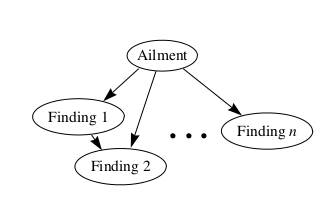
\includegraphics[scale=0.6]{figs/ailment.png}
	\caption{用于医学诊断的贝叶斯网络}    
	\label{fig:ailment}
\end{figure}


后验概率的标准是全局的,在某种意义上说它对所有可能的依赖都是敏感的。在诊断问题中,后验概率的标准对与症状间的关系是敏感的,就像疾病和症状间的依赖关系。假定我们观察的所有症状在D中,一个更合理的标准是局部的,也就是说他忽视症状间的依赖关系,只对疾病和症状间的依赖关系敏感。这个观察值的完整数据可以应用到所有的分类和回归问题中。


Dpiegelhalter (1993)提出了一个局部标准,就是在序列边缘函数标准下的
\begin{equation}
\label{eq:38}
LC(S^h,D)=\sum_{i=1}^N \log p(a_l| \boldsymbol{F}_l,D_l,S^h)
\end{equation}
其中$a_l$和$\boldsymbol{F}_l$代表疾病A的观察值和在第l个样例中的症状集$\boldsymbol{F}$。换句话说,为计算第l项,我们用前l-1个样例来训练模型S,然后根据第l个样例的症状来判断疾病。我们可以把这个标准当作训练样本和检验样本从未互换的交叉验证。


log效用函数有有趣的理论属性,但是有时候在现实问题中就是不正确。一般情况下,一个合适的评分或效用函数依赖于决策问题或应用了概率模型的问题。Howard and Matheson(1983)整理了一系列秒苏如何构建特殊决策问题的效用模型的文章。一旦我们构建了这个效用模型,我们可以修改公式\ref{eq:38}的形式来进行模型选择。



\section{边缘似然的计算}
就像之前提及的,常用模型选择的标准是对相关后验概率取对数$\log p(D,S^h)=\log p(S^h)+\log p(D|S^h)$。在这部分,我们讨论一下第二部分边缘似然$p(D|S^h)$的计算。


假定(1)局部分布函数属于指数家族,(2)参数$\theta_i$相互独立,(3)这些参数的共轭先验,(4)完整数据,那么边缘似然的对数可以有效的求解。公式\ref{eq:35}是一个非限制的多项式分布的例子。Buntine(1994)和Heckerman and Geiger(1996)讨论了其他局部分布函数的计算。这里,我们集中在不完整数据的近似。


当我们用不完整数据来计算边缘似然,用蒙特卡罗和高斯近似来学习我们在第六部分讨论的参数是很有用的。Chib(1995) and Raftery(1996)提出了一种蒙特卡罗方法,使用了贝叶斯理论
\begin{equation}
p(D|S^h)=\frac{p(\boldsymbol{\theta}_s|S^h)p(D|\boldsymbol{\theta}_s,S^h)}{p(\boldsymbol{\theta}_s|D,S^h)}
\end{equation}
对于$\boldsymbol{\theta}$的任何配置,分子上的先验项可以直接获得,此外,分子上的似然项可以通过贝叶斯网络推理计算得出。最后,分母上的后验项可以使用吉布斯采样计算而得,就像我们在6.1部分提及的。另外,更复杂的蒙特卡罗方法在DiCiccio et al(1995)中描述。


就想我们描述的,蒙特卡罗方法是正确的但是计算并不方便,特别是对于大数据。相反,基于高斯估计的方法更有效,并能在大数据集的处理上保持和蒙特卡罗相同的正确率。


回想一下,对于大量的数据,$p(D|\boldsymbol{\theta}_s,S^h)*p(\boldsymbol{\theta}_s|S^h)$经常近似于多维高斯分布。
\begin{equation}
\label{eq:40}
p(D|S^h)=\int p(D|\boldsymbol{\theta}_s,S^h)p(\boldsymbol{\theta}_s|S^h)\,d\boldsymbol{\theta}_s
\end{equation}
结果$p(D|S^h)$可以用类似的形式计算。特别地,将公式\ref{eq:31}代入到公式\ref{eq:40},并对结果取对数,我们得到近似值:
\begin{equation}
\log p(D|S^h) \approx \log p(D|\overline{\boldsymbol{\theta}}_s,S^h)+\log p(\overline{\boldsymbol{\theta}}_s|S^h)+\frac{d}{2}\log(2\pi)-\frac{1}{2}\log|A|
\end{equation}
其中d是$g(\boldsymbol{\theta}_s)$的维度。对于一个非限制的多项式贝叶斯网络,这个维度可以通过$\sum_{i=1}^n q_i(r_i-1)$给出。有时当模型中有隐藏变量时,此时维度会更低一点。Geiger(1996)讨论了这一点。


这种集成的评估技术被叫做拉普拉斯方法,我们也将公式\ref{eq:41}称为拉普拉斯评估。Kass(1988)提到,在一定规则条件下,这种评估的相关误差是$O(1/N)$级别的,其中N是样本D中样例的个数。因此,拉普拉斯评估可以说是相当精确的。对于这个评估方法更详细的讨论可以看这篇文章Kass(1988)和Kass and Raftery(1995)。



虽然拉普拉斯评估和蒙特卡罗方法紧密相关,但对于大维度模型,矩阵$|A|$的计算是相当密集的。一种简化评估矩阵$A$的方法是只使用海森矩阵$A$的对角线元素。一旦这样做了,也就是说我们认为参数之间是相互独立的,但是研究者发现这种评估在某些情况下是正确的(Becker and LeCun,1989 and Chickering and Heckerman,1996)。拉普拉斯的另一个变体是Cheeseman and Stutz(1995)提出的。他在自动分类程序中使用评估来进行数据聚类(Chickering and Heckerman,1996)。


我们通过保持公式\ref{eq:41}中的项而去增加N,从而获得一个有效的评估方法(但是不够非常准确):其中$\log p(D|\overline{\boldsymbol{\theta}}_s,S^h)$将会以线性增加,$\log |A|$将会以$d\log N$增加。同样,对于数值很大的N,$\overline{\boldsymbol{\theta}}_s$可以通过对$\boldsymbol{\theta}_s$配置的最大似然来评估。因此,我们获得
\begin{equation}
\label{eq:42}
\log p(D|S^h) \approx \log p(D|\overline{\boldsymbol{\theta}}_s,S^h)-\frac{d}{2}\log N
\end{equation}
这种评估叫做贝叶斯信息准则(BIC),该定义首次来自Schwarz(1978).



BIC评估在几个方面是有趣的。首先,它不依赖于先验。因此我没呢可以在不使用先验的情况下进行评估\footnote{来源于这种评估方法的一种技术假定是$\overline{\boldsymbol{\theta}}_s$非零}。第二,这种评估是相当靠直觉的。也就是说,它包含一个衡量参数化模型好坏的项来预测数据($\log p(D|\overline{\boldsymbol{\theta}}_s,S^h)$)以及一个惩罚模型复杂度的项($d/2\log N$)。第三,BIC评估是直接减去Rissanen(1987)提出的最小描述长度准则(MDL)。因此,回忆在第9部分的讨论,我们可知边缘似然提供了交叉验证和MDL之间的联系。


\section{先验}
为了计算一个网路结构相关的后验概率,我们必须评估结构先验$p(S^h)$和参数先验$p(\boldsymbol{\theta}_s)$(除非我们使用大样本估计,比如BIC/MDL)。在第八部分,参数先验$p(\boldsymbol{\theta}_s|S^h)$也是需要选择打分函数。不幸的是,当许多网络结构是不可能的,这些评估是无法追踪的。然而,在一定假设下,我们可以从一个易管理的直接假设的数中获得许多网络结构的结构和参数先验。几个作者讨论这个假定和获取先验的相关方法(Cooper and Herskovits,1991,1992;buntine,1991;Spiegelhalter et al,1993;heckerman et al,1995b;heckerman and Geiger,1996)。在这一部分,我们试验其中几个方法。


\subsection{网络参数的先验}
首先,让我们考虑一下网络结构中参数先验的评估。我们考虑由Heckerman et al(1995b)提出的方法:假定样例的局部分布函数是非限制的多项式分布并且参数是独立的。


该方法是基于两个关键的理论:独立等价和分布等价。如果对于变量集$\boldsymbol{X}$,两个贝叶斯网络结构有相同条件独立断言,那么这两个网络是独立等价的。比如,给定$\boldsymbol{X,Y,Z}$,网络结构$X \rightarrow Y \rightarrow Z,X \leftarrow Y \rightarrow Z,X \leftarrow Y \leftarrow Z$代表着唯一的断言X和Z在给定Y的条件下是独立的,所以这些结构是等价的。另一个例子是,一个完全的网络结构没有丢失的边,也就是说没有条件独立的断言。当$\boldsymbol{X}$包含n个变量,那么有$n!$个可能的完全网络结构:每个网络结构对应一个变量的排序。对于$p(x)$所有完全网络结构是独立等价的。一般,只有当他们有相同的结构(忽视弧方向)和相同的v结构(Verma and Pearl,1990),这两个网络结构才独立。v结构是一个有序的元组(X,Y,Z),其中X到Y有个弧,Z到Y有个弧,而X和Z之间没有弧。


分布等价的理论和独立等价很类似。假定对于变量集$\boldsymbol{X}$所构成的所有贝叶斯网络都具有在家族$\mathcal{F}$中的局部分布函数。这不是一个限制,因为$\mathcal{F}$可以是一个大家族。如果由变量集$\boldsymbol{X}$构成的贝叶斯网络结构$S_1$和$S_2$有相同的联合概率分布,也就是说对于每个$\theta_{s1}$存在一个$\theta_{s2}$使$p(x|\theta_{s1},S_1^h)=p(x|\theta_{s2},S_2^h)$,那么对于家族函数$\mathcal{F}$而言,它们都是分布独立的。


对于一些家族函数$\mathcal{F}$,分布等价也暗示着独立等价,但是相反缺不成立。比如,当$\mathcal{F}$是一般线性回归家族函数,那么对于超过3个变量的完全网络结构就不能代表相同的分布集合。然而,也有函数家族$\mathcal{F}$,独立等价也暗示着分布独立。比如非限制的多项式分布和携带高斯噪声的线性回归模型。



分布等价的观念是重要的,因为如果两个网络结构$S_1$和$S_2$对于给定的一个$\mathcal{F}$是分布等价的,那么和这两个结构相关的假说是一致的,也就是说$S_1^h=S_2^h$.因此,如果$S_1$和$S_2$是分布等价,那么他们的概率在任何信息状态下都是相等的。Heckerman et al(1995b)称这个属性叫假设等价。


根据这个属性,我们将每个假设和一个结构等价的类联系起来而不是一个单独的网络结构。我们学习网络结构的方法应该和学习等价的网络结构的类的方法是类似的(为了文章简短起见,我们通常模糊这个区别)。比如,在公式\ref{eq:33}中网络结构假设的和可以用等价类假设的和来替代。识别一个给定网络结构的等价类的算法在Chickering(1995)中提及。



我们注意到假设等价提供了我们解释贝叶斯网络结构为条件独立的表示。然而,贝叶斯网络的强定义使得弧有了因果推理(看第15部分)。Heckerman et al(1995b)和Heckerman(1995)认为虽然在处理因果贝叶斯网络时使用假设等价是不合理的,但是它对于似然等价的弱假设是合理的。也就是说数据库中的观察值不能帮助区分这两个等价的网络结构。



现在,让我们回到这部分的主题:从一个可管理的评定数据中获得先验。Geiger and Heckerman(1995)表示参数独立和似然等价的假设暗示了对于任何完全网络结构$S_c$的参数必须是狄利克雷分布,而且其超参有如下限制:
\begin{equation}
\alpha_{ijk}=\alpha p(x_i^k,pa_i^j|S_c^h)
\end{equation}
其中$\alpha$是用户等价的样本大小,而$p(x_i^k,pa_i^j|S_c^h)$是由用户的联合概率分布$p(x|S_c^h)$计算而来。这个结果是相当合理的,因为这两个假设导致限制的狄利克雷是合理的。


为了确定不完全网络结构参数的先验,Heckerman et al(1995b)使用参数模块化的假设,也就是如果$X_i$在网络结构$S_1$和$S_2$中有相同父节点,那么
\begin{equation}
p(\boldsymbol{\theta}_{ij}|S_1^h)=p(\boldsymbol{\theta}_{ij}|S_2^h)
\end{equation}
其中$j=1,\cdots,q_i$。这一属性被称为参数模块化,因为参数$\theta_{ij}$的分布只和网络的结构有关,准确的说是和$X_i$和它的父节点。



给定参数模块化和参数独立的假设,从给定先验的完全贝叶斯网络中构建任意网络结构的先验参数是个简单的问题。特别的,给定参数独立,我们分开对每个节点的参数构建先验。此外,如果节点$X_i$在给定的网络结构中有父节点$\boldsymbol{Pa}_i$,我们识别这个$X_i$有父节点的完整的网络结构,并且使用公式\ref{eq:43}和参数模块化来确定这个节点的先验。结果就是所有网络结构的所有项$\alpha_{ijk}$将会被公式\ref{eq:43}所确定。因此,由$\alpha$和$p(x|S_c^h)$,我们可以获得所有可能网络结构的参数先验。结合公式\ref{eq:43}和公式\ref{eq:35},我们可以获得一个模型选择准则,即将相等的边缘似然赋值给独立等价的网络结构。


我们可以通过构建一个贝叶斯网络来评估$p(x|S_c^h)$,这叫做先验网络,以此来描述联合分布。Heckerman et al(1995)讨论了这个网络的构建。


\subsection{结构的先验}
现在,我们来考虑一下在网络结构假设中对先验的评估。注意到在第八部分有选择的标准能够合并网络结构中的先验偏差。在这部分,相似的方法被用来评估这个偏差。


给网络结构的先验赋值的最简单的方法是假定每个结构出现的概率是相等的。当然,这种假设是不准确的,只是为了方便。这个方法的一种优化是让用户排除不同的假设(可能基于因果关系),然后根据剩余的假说给出统一的先验。我们在12部分介绍这个方法。


Buntine(1991)描述了一系列假定集来是方法更有效的得到先验。第一个假设是变量是有序的(知道了时间优先权)。第二个假设是有没有弧是相互独立的。在这些假定下,有$n(n-1)/2$可能的结果决定了任意一个可能的网络结构的先验概率。这种的方法的一个扩展是允许多种可能的排序。一种简化是假定有没有弧的概率是独立于特别的弧。在这种情况下,只要评估一个概率。


Heckerman et al(1995b)提出来另一个方法,它使用一个先验网络。基本想法是通过衡量结构和先验网络的相差程度来对先验概率进行”惩罚“。


Madigan et al(1995)也给了一种充分利用领域专家的想象数据方法。在他们的方法中,一个计算机程序帮助用户创建理想的完整数据集。然后,在给定数据和假定先验概率是一样的条件下使用像第七部分的方法来计算网络结构的后验概率。最后,他们把这个后验概率当先验对真实的数据进行分析。



\section{搜索方法}
在这部分,我们检测一些识别网络结构的搜索方法,这些方法按照一些准则来给网络结构打分。考虑这样一个问题,就是从一个网络集合中找出最好的网络,而这些网络中每个节点有不超过k个父节点。不幸的是,当我们使用公式\ref{eq:43}中限制的先验(Chickering et al,1995)时,那么$k>1$的问题就是个NP问题。因此,研究者使用启发式搜索算法,包括贪婪搜索,带重启的贪婪搜索,最佳最好搜索和蒙特卡罗方法。



令人安慰的是当这些模型选择标准可分时,这些搜索方法可以更有效。给定由变量集$X$构成的网络结构,如果它可以被写成变量乘积,那么我们所说的区分结构的准则是可分。
\begin{equation}
C(S^h,D)=\prod_{i=1}^n c(X_i,Pa_i,D_i)
\end{equation}
其中$D_i$是受限于变量$X_i$和父节点$Pa_i$的数据。可分准则的准则样例有BD准则(公式\ref{eq:34}和\ref{eq:35}),它使用






%\begin{table}[!hbp]%开始表格
%\caption{TABLE 1} %表格的名称
%\begin{tabular}{c c}%开始绘制表格
%\hline %绘制一条水平的线
%\textbf{Advantages} 			& 			\textbf{Disadvantages}				\\
%\hline
%Utilization increased  		&  			Performances degraded 				\\
%Live Backup and migrations  	&			No real standards					\\
%Cloning and snapshots  		&			storage								\\
%Energy saving   				&			Complex root cause analysis			\\
%Administration is easier  	&			New concepts and tools				\\
%-  							&			Low graphics							\\
%Go green						&			Multimedia performance - poor		\\
%Manage and monitor regulatory compliance		&		-						\\
%Flexibility and mobility		&			Peripheral support - poor			\\
%Reduced costs				&			Cannot work offline					\\
%Disaster recovery			&			Single point of failure (SPOF)		\\
%Data security				&			can’t virtualize just everything		\\
%Lower noise					&												\\
%\hline
%\end{tabular}
%
%\end{table}






%




\bibliographystyle{unsrt}										% 按引用的先后顺序排列,比较次序为作者,年度和标题
\bibliography{mybib}												% 引用文件数据库在bib.bib文件中

\clearpage     
\end{CJK*}

\end{document}